%!TEX root = ./Body.tex

\chapter{Features} % (fold)
\label{cha:Features}

\section{Strukturierung} % (fold)
\label{sec:Strukturierung}
Für die Feature-Extraktion-Process haben wir Feature-Vektoren für alle Referenz-Fahrt-Paare generiert (Siehe Abbildung ~\ref{fig:feature_extraction}). Diese Features wurden danach auch normalisiert, da es eine bessere numerische Stabilität ergibt und man kann auch die Ausreißer vermeiden. Ebenfals wurden die Features in eine Feature-Liste zusammengefast, um eine leichte Verarbeitung zu ermöglichen.

\begin{figure}[htbp]
\begin{center}
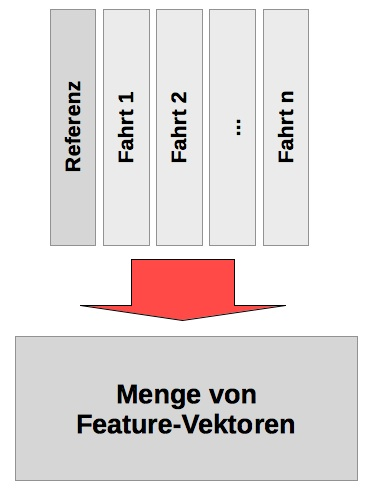
\includegraphics[width=0.4\textwidth]{feature_extraction}
\caption{Feature Extraktion}
\label{fig:feature_extraction}
\end{center}
\end{figure}

% section Strukturierung (end)


\section{Berechnung der benutzten Features} % (fold)
\label{sec:Berechnung_der_benutzten_Features}
So dass jeder die Features in der gleichen Weise benutzen könnte, wurde eine Werkzeug im Framework implementiert, um der Auswahl, der für Training relevanten Features, zu machen. Mittels diese Werkzeug war die Online-Bereitstellung der Features im Framework auch möglich. Die aufnehmende Daten wurden in Untermengen für Training, Test und Evaluation aufgeteilt.\\

Für unsere Feature-Raum haben wir die Zukunft und die Vergangenheit betrachtet (Siehe Abbildung ~\ref{fig:feature_vektoren}). Wir haben die Vektoren und die Winkeln zwischen die zeitliche verschiedene Fahrzeugspunkte und Trajektorienpunkte berechnet. In Abbildung  ~\ref{fig:feature_overview} ist eine Überblick über die Features.

\begin{figure}[htbp]
\begin{center}
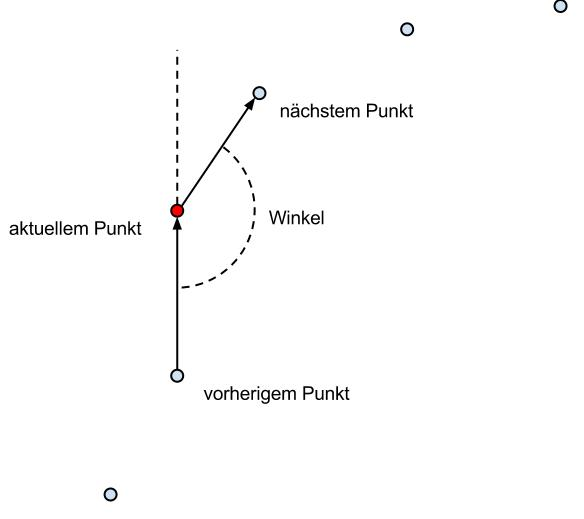
\includegraphics[width=0.6\textwidth]{feature_vektoren}
\caption{Vektoren}
\label{fig:feature_vektoren}
\end{center}
\end{figure}

\begin{figure}[htbp]
\begin{center}
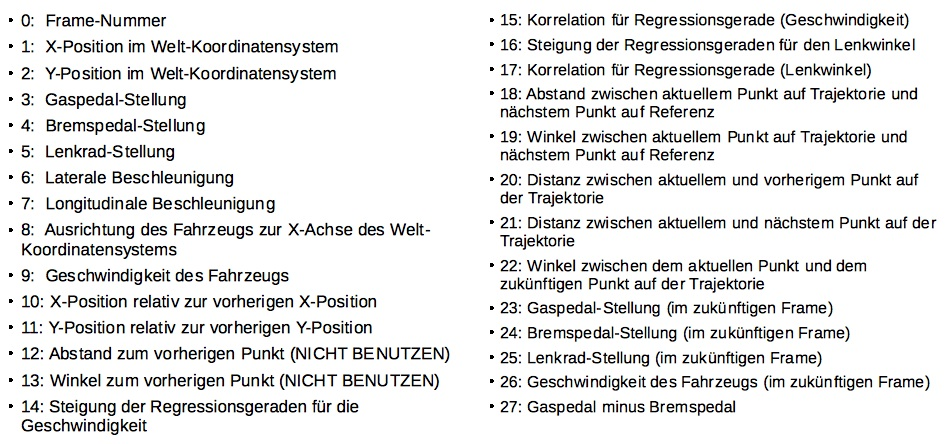
\includegraphics[width=1\textwidth]{feature_overview}
\caption{Feature Overview}
\label{fig:feature_overview}
\end{center}
\end{figure}
% section Berechnung_der_benutzten_Features (end)


\section{Vergleiche, Korrelation, Verwendete Features} % (fold)
\label{sec:Vergleiche_Korrelation}
Wir haben die Features analysiert, um Korrelationen zwischen denen und die Variablen (Gas, Bremse und Winkel des Lenkrads) zu finden. Dafür wurden viele Kombinationen ausprobiert. Siehe Abbildung ~\ref{fig:with-no-correlation} und ~\ref{fig:with-correlation} für ein paar Beispiele mit schlechte und gute Korrelation. Schließlich wurden die folgende Features für den Training benutzt.

\begin{itemize}
	\item 6: Laterale Beschleunigung
	\item 7: Longitudinale Beschleunigung
	\item 9: Geschwindigkeit des Fahrzeugs
	\item 18: Distanz vom Fahrzeug zum nächsten Punkt
	\item 19: Winkel vom Fahrzeug zum nächsten Punkt
\end{itemize}

\begin{figure}[htbp]
\begin{center}
\subfigure{\label{fig:feature_with-no-correlation-gas}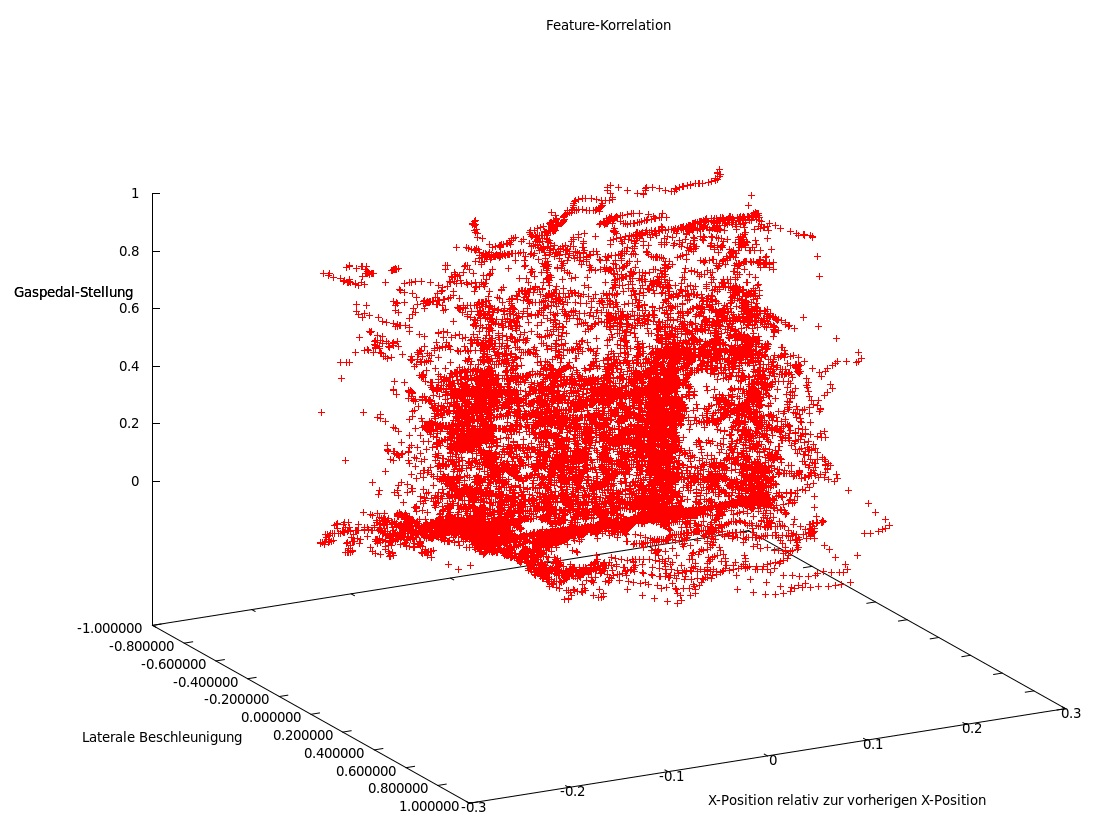
\includegraphics[width=0.45\textwidth]{feature_with-no-correlation-gas}}    
\hspace{1cm}            
\subfigure{\label{fig:feature_with-no-correlation-winkel}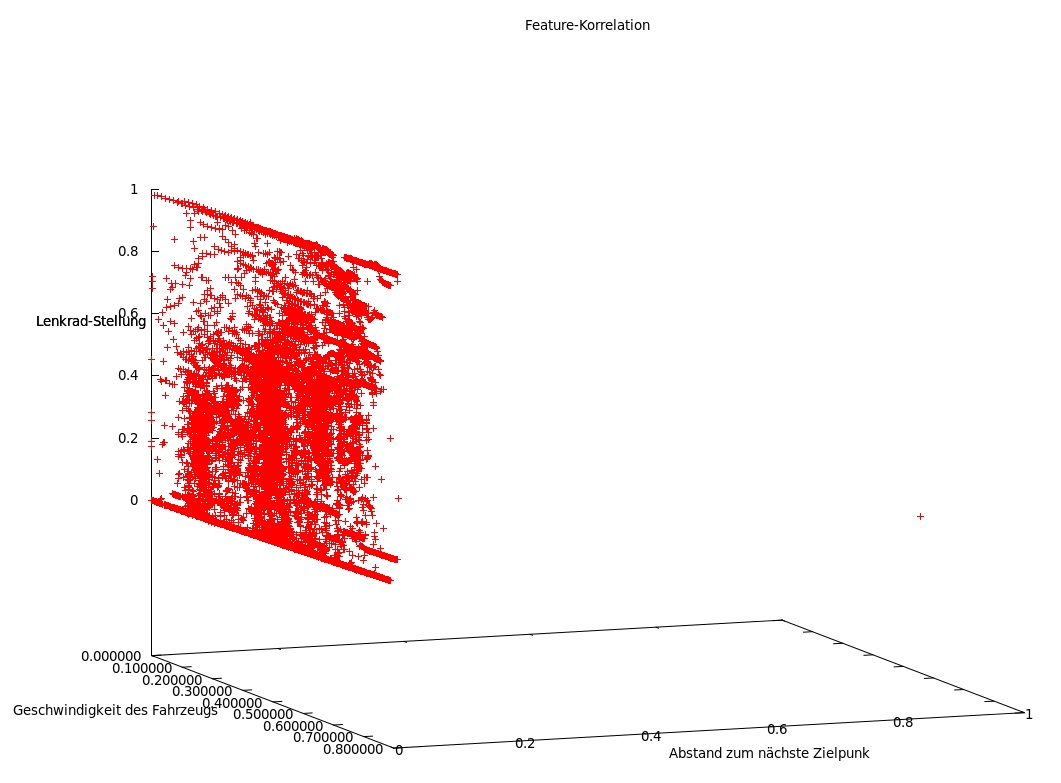
\includegraphics[width=0.45\textwidth]{feature_with-no-correlation-winkel}}
\caption{(a) Schlechte Korrelation mit Gas. (b) Schlechte Korrelation mit Winkel.}
\label{fig:with-no-correlation}
\end{center}
\end{figure}

\begin{figure}[htbp]
\begin{center}
\subfigure{\label{fig:feature_with-correlation-gas}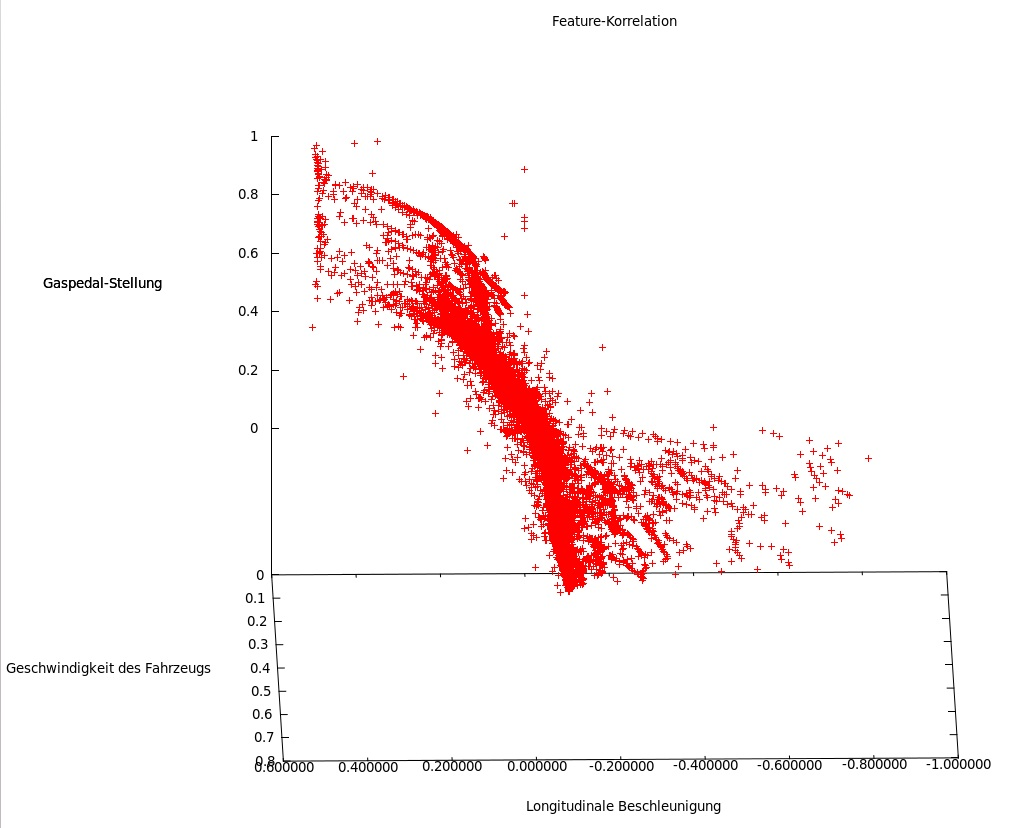
\includegraphics[width=0.45\textwidth]{feature_with-correlation-gas}}    
\hspace{1cm}            
\subfigure{\label{fig:feature_with-correlation-winkel}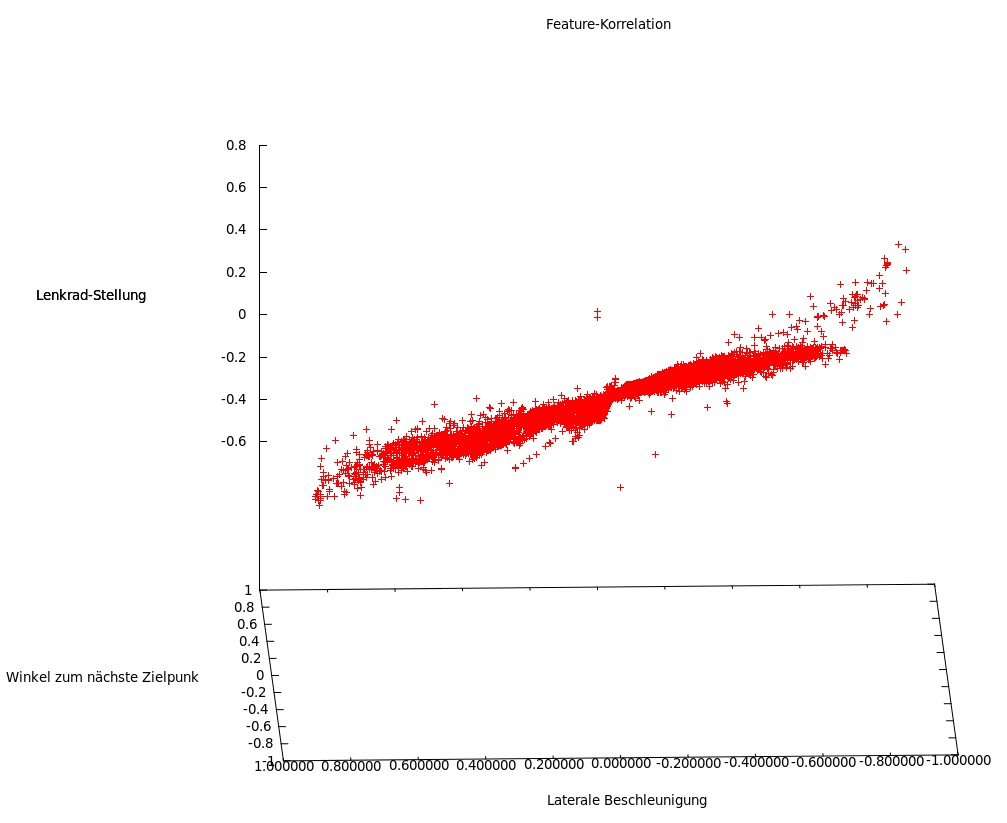
\includegraphics[width=0.45\textwidth]{feature_with-correlation-winkel}}
\caption{(a) Gute Korrelation mit Gas. (b) Gute Korrelation mit Winkel.}
\label{fig:with-correlation}
\end{center}
\end{figure}

% section Vergleiche_Korrelation (end)


% chapter Features (end)
